\documentclass[12pt]{article}
\usepackage{graphicx}
%\usepackage[a4paper,margin=1in]{geometry}
\usepackage{hyperref}
\usepackage{amsmath}
\usepackage{amssymb}
\usepackage[numbers, square, sort&compress]{natbib}
\usepackage{siunitx}
\usepackage{bm}

\title{Chapter 2: Conformations Search methods for molecular docking}
\author{Elvis Martis}
\begin{document}
\maketitle


\section{Basic concepts}
Understanding molecular conformation, the three-dimensional arrangement of atoms in a molecule, is fundamental to computational chemistry. A molecule’s conformation determines its chemical and biological properties, including reactivity, solubility, and binding affinity to biological targets. In the context of molecular docking, this conformational search is performed within the receptor's binding site to locate the bioactive conformation. Unlike global or local minimum conformations in solution, the bioactive conformation is a low-energy conformation that exhibits the most appropriate shape complementary to the binding site. This maximises favourable interactions between the ligand and receptor atoms. The success of structure-based drug design methods depends on identifying this bioactive conformation.

A typical small drug-like molecule may contain multiple rotatable bonds, each capable of adopting several energetically distinct conformational states. With $n$ rotatable bonds and approximately 3 accessible rotameric states per bond, the conformational space contains roughly $3^n$ distinct conformations. For a molecule with 12 rotatable bonds, typical for many pharmaceutically relevant compounds, this yields nearly 530,000 possible conformations. Manual identification becomes impractical, necessitating automated conformational search methods.

\subsection{Potential Energy Surface}

The potential energy of a molecule  is expressed as a function of the nuclear/atomic coordinates\cite{CH2_Jensen2017,CH2_Cramer2013} given by:

\begin{equation}
    \textrm{V}(\mathbf{\textrm{R}}) = \textrm{V}(\textrm{R}_1, \textrm{R}_2, \dots, \textrm{R}_{\textrm{{3N}}}),
    \label{eq:PES}
\end{equation}

where N is the number of atoms and $\mathbf{\textrm{R}}$ is the 3N-dimensional vector of Cartesian nuclear positions. For a non-linear molecule, the number of internal degrees of freedom is 3N - 6, after removal of overall translation and rotation. A potential energy surface (PES) can be defined as the hypersurface obtained by plotting $\textrm{V}(\mathbf{\textrm{R}})$ against a chosen set of internal coordinates (bond lengths, angles and torsions). Such high-dimensional PES cannot be visualised for human interpretation; therefore, we must restrict plotting to only a few important internal coordinates. These important internal coordinates, also known as collective variables, may be sufficient to explain the behaviour of the entire chemical or biochemical system. The n-butane systems offers a simple example of a PES(\textbf{Figure \ref{fig:confanalysis}}) plotted by rotating the central rotatable bond ($\textrm{C}_\textrm{2}$--$\textrm{C}_\textrm{3}$).

\subsubsection{Stationary points and the Hessian matrix}
While exploring the PES, the key parts we are most interested in are locating the energy minimum. Mathematically, minimum or maximum points on the PES are located by differentiating the force field function describing the chemical system. In an ideal system, the minimum (See points A and B in \textbf{Figure \ref{fig:confanalysis}}) or maximum (See points C and D in \textbf{Figure \ref{fig:confanalysis}}) is defined as a stationary point on the PES such that the first-order derivative of the function is zero and is classified by the eigenvalues of the Hessian matrix. The following equations illustrate this fact:
\begin{equation}
    \frac{\partial V}{\partial q_i} = 0
    \quad\textrm{for all internal coordinates }  q_i,
    \label{eq:PES_der}
\end{equation}

\begin{equation}
    \textrm{H}_{\textrm{ij}} = \frac{\partial^2 V}{\partial q_i,\partial q_j}
    \label{eq:PES_hamil}
\end{equation}

A local minimum has all positive eigenvalues (no imaginary frequencies), whereas a first-order saddle point (transition state) has exactly one negative eigenvalue (one imaginary frequency). The topology of the PES around these points controls conformational equilibria and reaction rates\cite{CH2_Jensen2017}.

\subsubsection{Energy profiles and reaction coordinates}

In one dimension, for example, rotation of a torsion angle, the PES reduces to an energy profile V(s) along a reaction coordinate (s) (\textbf{Figure \ref{fig:confanalysis}}) . Energy minima correspond to stable conformers, while barriers may correspond to transition structures. Such barriers also suggest the kinetic accessibility of conformational interconversion, as their heights determine the rate at which one conformer transforms into another. Low barriers enable rapid interconversion on short timescales, leading to dynamic averaging of conformations, whereas high barriers result in kinetically trapped states that may be experimentally distinguishable. Consequently, the shape of the energy profile not only defines the relative stability of conformers but also governs their population distribution and dynamical behaviour under given thermodynamic conditions\cite{CH2_wales2015perspective}.

\subsubsection{Internal coordinates}

For molecular mechanics representations, it is convenient to use internal coordinates such as:
\begin{itemize}
\item Bond stretches r,
\item Angle bends $\theta$,
\item Improper torsions $\chi$ (for planarity/chirality),
\item Proper torsions (dihedrals) $\phi$,
\end{itemize}

A generic functional form for the molecular mechanics potential energy is given by:

\begin{equation}
    V(\mathbf{q}) =
    \sum_\text{bonds} k_r (r - r_0)^2 +
    \sum_\text{angles} k_\theta (\theta - \theta_0)^2 +
    \sum_\text{torsions} V_\text{tor}(\phi) +
    V_\text{nonbonded}
    \label{eq:PES_MOL}
\end{equation}

where $V_\text{nonbonded}$ computes van der Waals and electrostatic interactions, and $V_\text{tor}(\phi)$ is the torsional potential. Practically, conformational search tools treat bond stretching and angle bending as hard components of a force field. In other words, they are usually treated as fixed. The conformational search and moving along the potential energy surface are achieved by rotating the torsion angles; hence, we describe this in more detail.

\subsubsection{Torsional potentials}

The torsional potential is commonly expressed as a Fourier series (\textbf{Equation \ref{eq:PES_Four}}) to represent the periodicity of bond rotation. Each term in the series reflects distinct symmetry and energetic contributions, determined from quantum-mechanical calculations or experimental measurements.

\begin{equation}\label{eq:PES_Four}
    V_\text{tor}(\phi) =
    \sum_{n} \frac{V_n}{2}\bigl[1 + \cos\bigl(n\phi - \gamma_n\bigr)\bigr]
\end{equation}

where $V_\text{n}$ are barrier heights, n the periodicity, and $\gamma_\text{n}$ phase offsets.

\begin{figure}[hbt!]

    \centering
    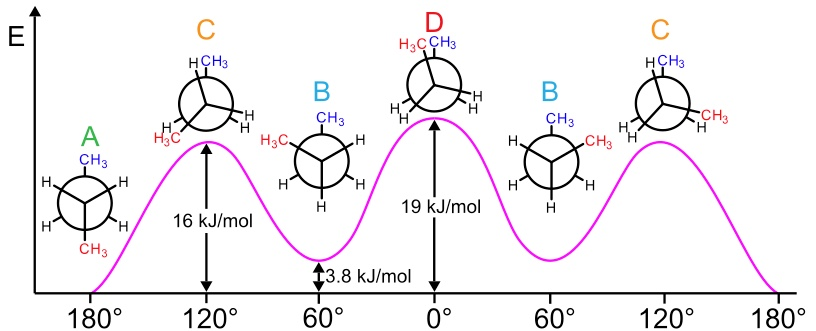
\includegraphics[width=1\textwidth]{conformations-of-butane.jpg}
    \caption{The Potential Energy Surface for simple molecular system, n-butane. The points A and B depict the low energy states (Gauche). The points C and D depict the high energy states (Eclipsed). The abscissa denotes the torsion angles ($\phi$), and the ordinate denotes the potential energy (E) of the system. This image is reproduced from \url{https://commons.wikimedia.org/} under the Creative Commons Attribution License (CC BY) licence.} 
    \label{fig:confanalysis}

\end{figure}

If we consider simple organic molecules:
\begin{itemize}
\item Ethane: $n = 3$, $\gamma = 0$, giving three equivalent staggered minima and three eclipsed maxima.
\item Butane: interplay between $n=3$ and $n=1$ terms to distinguish anti- and gauche-staggered minima (\textbf{Figure \ref{fig:confanalysis}}).
\end{itemize}

\subsubsection{Rotatable bonds}
Chemically, a rotatable bond can be defined as follows:

\begin{itemize}
\item A single (non-aromatic) bond ($\sigma$ bond) between heavy atoms
\item That is not in a ring
\item And is not terminal (i.e. not X–CH$_3$ or similar simple substituents)
\item Excluding amide C-N bonds, and other formally conjugated single bonds with high torsional barriers.
\end{itemize}


\section{Metrics to ensure conformational sampling}

\subsection{Energy-Based Metrics}

Key metrics characterise conformational search results:

\begin{equation}
    \Delta E = E_{\text{conformer}} - E_{\text{global minimum}}
\label{eq:relative_energy}
\end{equation}

The relative energy $\Delta E$ expresses each conformation’s energy relative to the lowest-energy structure. The Boltzmann population at temperature T predicts the probability of observing a particular conformation:

\begin{equation}
    P_i = \frac{e^{-\Delta E_i / k_B T}}{\sum_j e^{-\Delta E_j / k_B T}}
\label{eq:boltzmann}
\end{equation}

where $k_B$ is Boltzmann’s constant (1.987 cal·mol$^{-1}$·K$^{-1}$). At 298 K, conformations within 2 kcal/mol of the global minimum constitute $>10$ of the population and should be included in conformational ensembles.  The denominator is the \emph{partition function}, which serves as the normalisation factor that converts relative Boltzmann weights into physically meaningful probabilities.
Computational workflows, therefore:

\begin{itemize}
\item Sample a sufficiently diverse ensemble on the PES (system- and method-dependent).
\item Reweight or rescore conformers with higher-level methods when needed.
\item Consider entropic contributions associated with loss of conformational freedom upon binding.
\end{itemize}


\subsection{Structure-Based Metrics}
The RMSD quantifies geometric similarity between two conformations:

\begin{equation}
    \text{RMSD} = \sqrt{\frac{1}{N} \sum_{i=1}^{N} d_i^2}
\label{eq:rmsd}
\end{equation}

where $d_i$ represents the distance between atoms $i$ after optimal superposition. RMSD thresholds (typically 1.0–2.0 \r{A}) filter redundant conformations in search output.

\section{Conformational search methods}
One of the most challenging aspects of pose prediction is the conformational search algorithm. In general, there are two main classes of conformational search methods, systematic and stochastic.  Users do not always have the option to select the search algorithm, as developers usually choose based on their expertise and coding experience. Nevertheless, programs such as AutoDock allow users to select the search algorithm.

\subsection{Systematic Methods}
The systematic search algorithm rotates all possible rotatable bonds by a fixed interval. Such a method can explore all possible conformations; however, the complexity increases exponentially with the number of rotatable bonds. There are pruning algorithms that act as “bump check”, ruling out torsion angles that lead to significant atomic overlaps. The deterministic nature of systematic sampling ensures that the same input yields the same set of conformers, which is advantageous for benchmarking and reproducibility. However, the combinatorial explosion of grid points with increasing rotatable bonds quickly becomes prohibitive, especially for highly flexible ligands, motivating the use of hybrid schemes or coarse‑grained grids in practice\cite{CH2_Beusen1996,CH2_Leach2001}.

\subsubsection{Grid-based enumeration}

The simplest systematic approach divides torsion angle space into discrete intervals (e.g., 10° or 30°) and evaluates all possible combinations. For a molecule with $n$ rotatable bonds and 36 intervals per 360° rotation:


\begin{equation}
    N_{\text{conformations}} = 36^n
\label{eq:grid_enumeration}
\end{equation}

This method guarantees finding the global minimum but becomes computationally prohibitive for large $n$ (combinatorial explosion). Grid enumeration works well for rigid molecules with 2--4 rotatable bonds, but is impractical for flexible compounds.

In molecular docking, the search space is limited to the binding pocket, which is often represented as a grid. Therefore, the systematic conformational search engine operates by discretising the relevant degrees of freedom, typically torsional angles, on a grid.  It then generates and evaluates all combinations of torsion angles within that grid. For a molecule with n rotatable bonds, each torsion is sampled at a fixed interval, producing a Cartesian product of values  $\phi_1 \in {\phi_1^{(1)}, \dots, \phi_1^{(k)}}, \phi_2 \in {\phi_2^{(1)}, \dots, \phi_2^{(k)}}$ and so on. At each grid point, the geometry is energy-minimised, and the resulting conformers are clustered and ranked by energy or empirical scoring functions. Because the search is exhaustive within the chosen resolution, systematic methods can in principle locate all sterically allowed conformations of a given molecule, provided the grid is sufficiently fine, and the force field adequately describes the intramolecular energetics\cite{CH2_Ferreira2015}.

\subsubsection{The Z method}
The Z method\cite{CH2_Petrella2011} is a variant of grid-based conformational search protocols that uses statistical information about rotamers. It partitions the conformational space into subspaces and then applies repeated, uniform changes to a common starting structure, generating large ensembles of trial conformations in parallel. This approach enables rigid, systematic searches in high-dimensional spaces by combining grid-based sampling with statistical information from rotamer libraries. The Z Method can also be used hierarchically: low-resolution searches identify approximate regions of interest, which are then refined with finer grids or energy minimisation protocols. The key advantage is the ability to couple systematic search with probabilistic rotamer preferences, improving the sampling efficiency while preserving the exhaustiveness of the underlying grid. However, to the best of our knowledge, this method has only been applied to protein structure refinement. We did not find any literature references indicating its use as a conformational search tool for small molecules or in molecular docking.

\subsection{Fragment-based method}

In this method, the molecule is broken down into individual fragments\cite{CH2_sadowski2003conformational}. The fragments are then docked in the most suitable sub-pocket in the binding site. The entire molecule is then sequentially built by adding the linkers. This follows a systematic search for the linker conformation that optimally holds the fragments in their respective sub-pockets. The fragmentation method selects rigid molecular components, such as ring structures, as fragments and flexible components as linkers. In doing so, this method reduces computational complexity compared to a systematic search by focusing on small components, particularly the linkers. FlexX and DOCK are examples of the docking algorithms that employ this method as their conformational search algorithm.

\subsection{Stochastic Methods}
Stochastic techniques utilise random sampling and probabilistic methods to explore the conformational space. They work by randomly making changes, preferably to rotatable bonds, and evaluating the energy after each change. Metropolis Monte Carlo and the Genetic algorithm are popular stochastic search methods used as conformational search tools in docking programs.

\subsubsection{Monte Carlo}

It works on the principle of random sampling over a predetermined number of iterations to locate the optimal conformation\cite{CH2_Metropolis1953}. The search algorithm starts by making a random change in any of the randomly selected rotatable bonds. Following this, it evaluates the energy and compares it with the starting conformation. If the energy of the new state is lower than the previous state, then the conformation is accepted. If the energy of the new state is higher than that of the previous state, it assigns a random number between 0 and 1 and evaluates it against the Boltzmann distribution; if the random number is greater than the probability, the new state is accepted; otherwise, it is rejected. In case of rejection, the algorithm restarts from the previous conformations. The Glide docking program also employs Monte Carlo simulation in its docking algorithm to improve pose prediction accuracy.

In Metropolis Monte Carlo\cite{CH2_Metropolis1953}, a trial move from configuration  \(\mathbf{x}\) to \(\mathbf{x}'\) with energy change \(\Delta E = E(\mathbf{x}') - E(\mathbf{x})\) is accepted with probability
\begin{equation}
    P_{\mathrm{acc}}(\Delta E;T) =
    \begin{cases}
        1, & \Delta E \le 0, \\
        \exp\!\left(-\dfrac{\Delta E}{k_{\mathrm{B}} T}\right), & \Delta E > 0.
    \end{cases}
      \label{eq:MC_accept}
\end{equation}
At high T, uphill moves are readily accepted, enabling broad exploration of conformational space; as T is lowered, the algorithm increasingly favours low-energy states, mimicking physical annealing \cite{CH2_Kirkpatrick1983}.

\subsubsection{Genetic Algorithm (GA)}

Genetic algorithms are population-based metaheuristics motivated by biological evolution.\cite{CH2_Judson1993,CH2_Goodman1998} A GA iteratively evolves a population of conformers under the action of selection, crossover, and mutation, guided by a fitness function (typically related to energy or docking scores).

A basic GA cycle for conformational search is:

\begin{enumerate}
\item Initialisation: Generate an initial population of conformers (e.g., random torsion angles rotation).
\item Evaluation: Compute a fitness value for each conformer using an energy function.
\item Selection: Select parent conformers with probability biased toward higher fitness (e.g., tournament selection, roulette wheel).
\item Variation: Apply crossover and mutation operators in torsion space to generate offspring conformers.
\item Local optimisation: Perform local geometry minimisation to relax each offspring to the nearest local minimum.
\item Replacement: Form the new population from parents and offspring (e.g., generational or steady-state replacement, elitism).
\item Termination: Stop when convergence criteria are met (e.g., fixed number of generations, no improvement, or conformational coverage saturation).
\end{enumerate}

A critical design choice is how to encode conformations as chromosomes. For small molecules, a common representation is a vector of torsion angles:

\begin{itemize}
\item Each gene corresponds to a rotatable single bond, double bond stereochemistry, or ring-pucker degree of freedom.
\item The allele is a torsion angle (continuous, typically in $(-\pi, \pi)$), or a discrete bin for that torsion.
\item Chirality and double-bond E/Z configuration can be treated as additional discrete variables if the configurations are allowed to vary.
\end{itemize}

\subsection{Molecular Dynamics Simulations}

Molecular dynamics (MD) simulates the atomic motions as a function of time by solving Newton’s equations of motion.  MD simulations and molecular docking are complementary\cite{CH2_guterres2020improving} that are commonly employed in structure-based drug discovery to understand the protein-ligand interactions and their dynamic aspects. For computational efficiency, molecular docking algorithms treat receptor rigidly and the ligand as flexible. This leads to incorrect pose prediction when induced-fit binding is observed\cite{CH2_salmaso2018bridging}. Therefore, MD simulation is an elegant method for incorporating such induced-fit effects. This can be achieved in two ways, as shown below:

\begin{itemize}
\item Pre-docking step to sample various conformations of the receptor without the influence of the ligand.  This can serve as multiple receptor conformations for docking.
\item Post-docking step to refine the docked receptor-ligand conformation by allowing the complex to evolve to its realistic conformation, which would be more probable physiologically.
\end{itemize}

A full chapter is dedicated to MD and methods based on it for post-processing and enhancing the sampling of receptor-ligand dynamics (see \textbf{chapter 9}).

\subsection{Simulated Annealing}

Simulated annealing (SA) is a concept more prevalent in engineering, where the malleability of metals/alloys is used to manufacture cables for a wide variety of applications. For example, a long steel cable can be manufactured from a block of steel by heating, beating, and cooling. This cycle is repeated until the desired shape, size and length is achieved, which dictates the tensile strength of the steel cable. This \emph{heating-beating-cooling} cycle is simulated annealing. Heating increases the steel's softness by allowing its atoms to move farther apart and gain kinetic energy. Thus, making the beating process easier and preventing any fracture or permanent deformation. The cooling stage traps the atoms in the beaten state. At the end of each cycle, the steel block progressively approaches the desired shape and size without losing its inherent steel properties. This idea can be implemented as a powerful stochastic optimisation technique\cite{CH2_Kirkpatrick1983}, widely used in conformational search for molecular docking, where the goal is to locate low‑energy ligand and protein conformations compatible with experimental binding modes. The heating in this case meant increasing the atoms' velocity so they could surmount the nearest energy barrier. Similarly, the cooling step reduced the velocity, so that the system now falls into the nearest local minimum. The heating and cooling are carried out iteratively to ensure maximum sampling of the PES. This mapping of thermodynamic annealing onto conformational space makes SA particularly suited to global-optimisation problems such as flexible‑ligand docking, where the search space is rugged and high‑dimensional\cite{CH2_Ghose1993,CH2_Naidoo1997,CH2_Corcho2000}.

The conceptual basis of SA is the Boltzmann distribution for a system with energy E at temperature T.
The equilibrium probability of a configuration with energy (E) is
\begin{equation}
    p(E;T) \propto \exp\!\left(-\frac{E}{k_{\mathrm{B}} T}\right)
    \label{eq:BOLTZ_PROB}
\end{equation}
where $\textrm{k}_{\mathrm{\textrm{B}}}$ is the Boltzmann constant. 

\begin{enumerate}
\item \textit{Heating phase}: Starting from an initial conformation, the system is rapidly heated to high temperature (typically 800–1000 K), providing energy to overcome conformational barriers.
\item \textit{Annealing phase}: Temperature is gradually reduced according to a cooling schedule, allowing the system to explore broader conformational space while progressively favouring lower-energy structures.
\item \textit{Minimisation phase}: At low temperature (50–100 K), geometry optimisation drives the system to a nearby local minimum.
\end{enumerate}

The SA protocol may be repeated several times from different initial conformations, generating diverse low-energy structures. Effectiveness depends on the cooling rate: too rapid cooling traps the system in local minima, while too slow cooling demands excessive computation.

\subsection{Distance Geometry Methods}

Distance geometry (DG)\cite{CH2_crippen_havel_book,CH2_havel_kuntz_crippen_1983,CH2_crippen_chem_dg_1991} provides an alternative formulation of conformational search in terms of interatomic distances rather than Cartesian coordinates. The central idea is to work in distance space: define lower and upper bounds on selected interatomic distances. Then complete these to a full metric that is (approximately) realisable in 3D Euclidean space. The metric is then embedded back into Cartesian coordinates. This approach leads to efficient generation of diverse, approximately low-energy conformations using only geometric information and modest energetic refinement.\cite{CH2_spellmeyer_dg_conf_1997,CH2_riniker_landrum_2015}

\subsubsection{Molecular distance geometry}
The molecular distance geometry problem (MDGP)\cite{CH2_crippen_chem_dg_1991,CH2_havel_dg_review_1998} formalises molecular conformation generation as follows:

Let $G = (V,E)$ be a graph whose vertices $V = {1,\dots,n}$ correspond to atoms. For each edge $(i,j) \in E$ we are given a distance interval

\begin{equation}
    \ell_{ij} \leq d_{ij} \leq u_{ij}
      \label{eq:Mol_DG}
\end{equation}
where $d_{ij}$ is the (unknown) true distance between atoms $i$ and $j$, and $\ell_{ij}, u_{ij} \ge 0$ are lower and upper bounds derived from e.g. ideal bond lengths, angle geometry, van der Waals radii, NMR restraints, or crystallographic data.

Find coordinates $\bm{x}_1,\dots,\bm{x}_n \in \mathbb{R}^3$ such that
\begin{equation}
   \ell_{ij} \le ||x_i - x_j|| \le u_{ij}, \quad \forall (i,j) \in E,
\label{eq:mdgp}
\end{equation}
and specified chirality constraints for selected quadruples of atoms are satisfied.

For small molecules, E typically includes:
\begin{itemize}
\item covalent bonds (tight bounds from ideal bond lengths),
\item 1–3 and 1–4 distances derived from bond angles and torsion ranges,
\item selected nonbonded distances (e.g. minimum separations to avoid clashes),
\item optional experimental distances (e.g. NMR NOEs) when available.
\end{itemize}

A single molecule usually yields several solutions to \textbf{Equation \ref{eq:mdgp}}, corresponding to different conformers. Therefore, conformational search using distance geometry focuses on sampling the feasible region defined by the aforementioned constraints, followed by force field optimisation and clustering.\cite{CH2_spellmeyer_dg_conf_1997,CH2_riniker_landrum_2015}

\subsubsection{Classical Distance Geometry Algorithm for Conformer Generation}

The standard DG pipeline in chemical applications, sometimes referred to as the EMBED algorithm and its variants\cite{CH2_havel_kuntz_crippen_1983,CH2_havel_dg_review_1998,CH2_spellmeyer_dg_conf_1997}, consists of three major stages:
\begin{enumerate}
\item \textit{Bound smoothing}: Given initial bounds on a sparse set of distances, bound smoothing propagates these constraints to non-neighbouring atom pairs using metric inequalities.
The simplest are triangle inequalities:
\begin{equation}
    d_{ik} \le d_{ij} + d_{jk}, \qquad
    d_{ik} \ge |d_{ij} - d_{jk}|
\label{eq:Bound_smoothing}
\end{equation}
which lead to tightened upper and lower bounds $u_{ik}$ and $\ell_{ik}$ when $d_{ij}$, $d_{jk}$ are themselves bounded. Computationally, the triangle-based smoothing method reduces to an all-pairs shortest path problem on a suitably constructed weighted graph.This can be implemented in $\mathcal{O}(n^3)$ time or better for sparse molecular graphs\cite{CH2_havel_kuntz_crippen_1983,CH2_havel_dg_review_1998}.

\item \textit{Embedding}: After smoothing, one obtains approximate lower and upper bounds $\ell_{ij},u_{ij}$ for all $i,j$. A specific target distance matrix D is then sampled by choosing each $D_{ij}$ uniformly or normally within $[\ell_{ij},u_{ij}]$, subject to symmetry and zero diagonal. Embedding proceeds via the metric matrix,
\begin{equation}
    B = -\frac{1}{2} J D^{(2)} J
  \label{eq:DG_embedd}
\end{equation}
If B is exactly positive semidefinite matrix with rank B $\le$ 3, then it corresponds to an exact Euclidean distance matrix (EDM) in $\mathbb{R}^3$ and the coordinates follow from the eigen-decomposition as above.

\item \textit{Refinement}: Refinement improves the geometrical consistency and the energy of the embedded structure.
A standard choice is to minimise a DG error function
\begin{equation}
 E(\{\bm{x}_i\}) =
 \sum_{(i,j)\in E} w_{ij}
 \left[
  f(d_{ij}(\{\bm{x}_i\}); \ell_{ij}, u_{ij})
 \right]^2
   \label{eq:DG_refine1}
\end{equation}

where $d_{ij}(\{\bm{x}_i\}) = \|\bm{x}_i - \bm{x}_j\|$ and $f$ penalizes deviations outside the allowed interval, e.g.
\begin{equation}
 f(d;\ell,u) =
 \begin{cases}
  d - u, & d > u,\\
  \ell - d, & d < \ell,\\
  0, & \text{otherwise}.
 \end{cases}
   \label{eq:refine2}
\end{equation}

Weights $w_{ij}$ can reflect confidence in the underlying constraints (for example, high for covalent geometry, lower for heuristic nonbonded bounds)\cite{CH2_crippen_chem_dg_1991,CH2_havel_dg_review_1998}.

Optimisation of E is typically performed using local methods, such as conjugate gradients, quasi-Newton methods, or simulated annealing. For small molecules, it is customary to combine DG error terms with a molecular mechanics force field:

\begin{equation}
    E_{\text{tot}} = E_{\text{DG}} + \lambda E_{\text{FF}},
  \label{eq:DG_OPT}
\end{equation}

with $\lambda$ chosen to balance strict adherence to DG constraints against optimisation of a realistic potential\cite{CH2_spellmeyer_dg_conf_1997}. This helps correct artefacts such as distorted aromatic rings or planar sp$^2$ centres that can arise in purely distance-based embeddings\cite{CH2_riniker_landrum_2015}.
\end{enumerate}


\section{Practical Considerations}

\subsection{Conformational flexibility in acyclic systems}

For simple alkanes, conformational preferences are well rationalised by
\emph{Newman projections}:
\begin{itemize}
\item Staggered conformers minimise torsional strain and often benefit from
hyperconjugative stabilisation.
\item Eclipsed conformers are higher in energy due to torsional and sometimes
steric/electrostatic repulsions.
\end{itemize}

In butane, the anti-staggered conformer is lowest in energy(\textbf{Figure \ref{fig:confanalysis}}), with the gauche conformers slightly higher but still populated at room temperature; this basic model generalises to many drug-like substituents.

Hyperconjugation and stereoelectronic effects (e.g., the gauche effect,
anomeric effect) often bias torsional preferences away from purely steric
expectations. These effects are naturally captured in quantum chemical PES
scans and, when parametrised appropriately, in modern force fields.

\subsection{Conformational flexibility in ring systems}

\subsubsection{Ring strain components}

Cycloalkanes illustrate several types of strain:
\begin{itemize}
 \item \textit{Angle strain}: deviation of bond angles from the ideal tetrahedral value (\(\approx\SI{109.5}{\degree}\)).
    \item \textit{Torsional strain}: eclipsing interactions between neighbouring bonds.
    \item \textit{Steric (non-bonded) strain}: 1,3-diaxial interactions, transannular repulsions in medium/large rings, etc.
\end{itemize}
Small rings (cyclopropane, cyclobutane) are strongly angle- and torsionally strained; cyclopentane relieves torsional strain by puckering; cyclohexane adopts near-strain-free conformations.

\subsubsection{Cyclohexane: chair, boat and twist-boat}

In cyclohexane, the most important conformations are:
\begin{itemize}
\item Two equivalent chair conformers, related by a ring flip.
\item Higher-energy boat and twist-boat conformations.
\end{itemize}

In the ideal chair, all C–C bonds are staggered, and the internal bond angles are close to tetrahedral. A ring flip exchanges axial and equatorial positions; for monosubstituted cyclohexanes, the equilibrium strongly favours the equatorial conformer for bulky substituents due to reduced 1,3-diaxial repulsions.

From a computational perspective, the PES in the relevant ring-puckering coordinates shows:
\begin{itemize}
\item Two deep minima (chairs),
\item A pathway via twist-boat and boat conformations connecting them,
\item Barriers that set the timescale for ring inversions.
\end{itemize}

\subsubsection{Conformational analysis of substituted and heterocyclic rings}

Substitution and heteroatoms modify ring conformations and relative energies:

\begin{itemize}
\item Electronegative or $\sigma$-accepting substituents can introduce stereoelectronic effects (e.g.\ anomeric effect in pyranoses).
\item Heteroatoms alter bond lengths/angles, and their steric profiles, thereby altering A-values (axial penalty) and flipping preferences.
\item Fused ring systems transmit conformational bias conformational transmission, important in polycyclic scaffolds used in medicinal chemistry.
\end{itemize}
Accurate treatment of these systems often requires a combination of high-quality force fields and validation against quantum-chemical PES scans or experiments.

\subsection{Accounting for solvation effects}

Bioactive conformations depend on the solvent environment. Implicit solvation models (Generalised Born, Poisson-Boltzmann) add solvation energy terms, affecting the conformational landscape relative to gas-phase calculations.

\subsection{Validation Metrics}

Conformational search quality is evaluated by:

\begin{enumerate}
\item \textit{Recovery of Crystallographic Conformations}: For validation datasets with known bioactive structures (e.g., protein-bound ligand conformations), the minimum RMSD from the ensemble to experimental structure indicates success. Recovery within 2 \r{A} RMSD is considered good.

\item \textit{Conformational Diversity}: The range of geometries in the final ensemble should comprehensively represent the conformational space. Metrics include the distribution of dihedral angles and the range of relative energies.

\item \textit{Computational Efficiency}: Wall-clock time and peak memory usage relative to molecular size determine practical viability. In drug discovery pipelines that screen millions of compounds, efficiency is paramount.
\end{enumerate}

\section{Summary}
Conformational search is the computational engine that enables docking. Understanding both the physics of the scoring function and the algorithms used to explore conformational space is essential for reliable predictions. Hybrid strategies that combine stochastic global exploration with local refinement currently offer the best trade-off between efficiency and accuracy.

\bibliographystyle{unsrtnat}
\bibliography{chapter2}

\end{document}